


\begin{document}

This report describes the design, implementation and test of an LED (light emmitting diode) driver. 

\noindent This report describes design, implementation and test of an LED driver comprised of a ring oscillator, schmitt trigger, and a current driver. The ring oscillator is comprised of complementary metal oxide semiconducting field effect transistors (CMOS) inverters connected in series. Figure \ref{fig:blockdiagram2} demonstrates where in the optical uplink project the LED driver is placed. 



\begin{figure}[H]
    \centering
    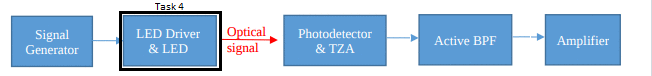
\includegraphics[width=.9\textwidth ]{Introduction/Block_Diagram_MFBP.png}
    \caption{Block diagram for optical uplink \cite{b1}}
    \label{fig:blockdiagram2}
\end{figure}


The LED driver circuit supplies the LED with a controlled current. A voltage driven output to light the LED is not used due to increased sensitivity from temperature change. 



\end{document}